
\begin{aufgabe}
	\begin{enumerate} [a)]
		\item Zeichnen Sie in die linke Skizze die Ihnen bekannten Kräfte ein.
		\item Lesen Sie sich das Wechselwirkungsgesetz noch einmal genau durch und zeichnen Sie in die rechte Skizze die Reaktionskräfte ein.
		\item Welche Kräfte wirken auf den Block?
	\end{enumerate}

	\begin{center}
	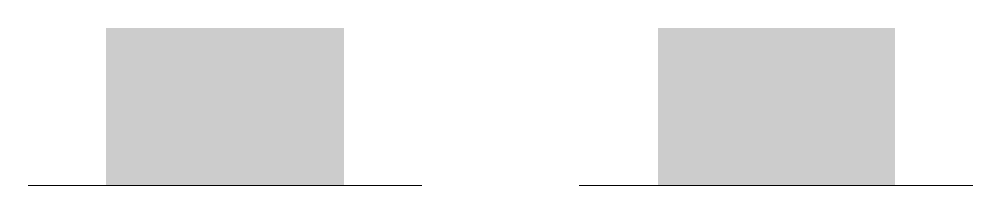
\begin{tikzpicture}
		\draw [fill, color=black!20] (1,0) rectangle(4,2);%box
\draw (0,0)--(5,0);%boden

%das gleiche noch einmal verschoben 
\begin{scope}[xshift=7cm]
\draw [fill, color=black!20] (1,0) rectangle(4,2);%box
\draw (0,0)--(5,0);%boden

\end{scope}
	\end{tikzpicture}
	\end{center}
\end{aufgabe}
